%%%%%%%%%%%%%%%%%%%%%%%%%%%%%%%%%%%%%%%%%%
\chapter{Heat transfer in packed beds} \label{ch:modeling-heat-transfer}
%%%%%%%%%%%%%%%%%%%%%%%%%%%%%%%%%%%%%%%%%%
This section covers a discussion of different modes of heat transfer experienced by a pebble in a packed bed. The main modes are conduction to neighbors and convection.




\section{Single particle modes of heat transfer}

\begin{figure}[t]
	\centering
	\caption{Each ceramic pebble in a fusion reactor will experience multiple modes of heat transfer.}
	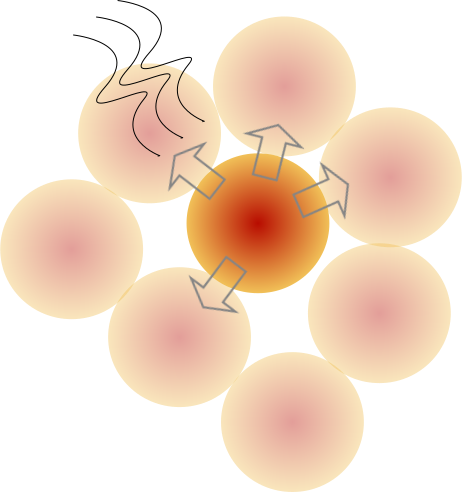
\includegraphics[width=0.75\textwidth]{chapters/figures/pebble-complete-heat-transfer}\label{fig:peb-comp-ht}
\end{figure}

The transient energy balance for an irradiated pebble, shown in Fig.~\ref{fig:peb-comp-ht}, in a packed bed with flowing interstitial gas is given by Eq.~\ref{eq:single-pebble-energy},

\begin{equation}\label{eq:single-pebble-energy}
	\rho V C \frac{\mathrm{d}T}{\mathrm{d}t} = \dot{Q}_g + \dot{Q}_\text{conduction} + \dot{Q}_\text{convection} + \dot{Q}_\text{radiation}
\end{equation}

We begin with the lumped capacitance assumption that internal temperature gradients inside of the solid particle are negligible thus we can neglect diffusion terms in the solid. The validity of that assumption for the ceramic pebbles in fusion reactors will be discussed in detail in \S\ref{sec:ht-jeffreson-correction}. The terms on the right-hand-side of Eq.~\ref{eq:single-pebble-energy} are:

\begin{enumerate}
\item Conduction through the stagnant fluid between two point- or non-contacted particles.
\item Conduction through the stagnant fluid between two area-contacted particles.
\item Conduction through the contact area between two area-contacted particles.
\item Conduction through the fluid in void space. 
\item Radiation between the surfaces of two particles.
\item Radiation between adjacent voids.
% \item Convective heat transfer between fluid and solid particles.
% \item rate of energy generated internal to the pebble,
% \item rate of conduction between neighboring pebbles in their regions of contact, 
% \item rate of convective heat transfer with the interstitial helium gas (which includes energy carried far downstream or redeposited to neighboring pebbles), and
% \item rate of radiative exchange between local solids.
\end{enumerate}

% In this section we will provide a brief overview of all the modes of heat transfer to provide an overview of the importance and impact of each mode. For cases when more detail is needed, the details will be expounded in their own complete sections.

% \subsection{Heat generation}

% Nuclear deposition of energy is handled in a straightforward manner. With a known volumetric energy generation rate, $q'''$ prescribed by, for instance, the neutron heating in the volume, the heat generation rate for this particle is simply

% \begin{equation}
% 	\dot{Q}_g = q'''V
% \end{equation}




%%%%%%%%%%%%%%%%%%%%%%%%%%%%%%%%%%%%%%%%%%
%\section{Single particle heat transfer}

\begin{figure}[t]
	\centering
	\caption{Each ceramic pebble in a fusion reactor will experience multiple modes of heat transfer.}
	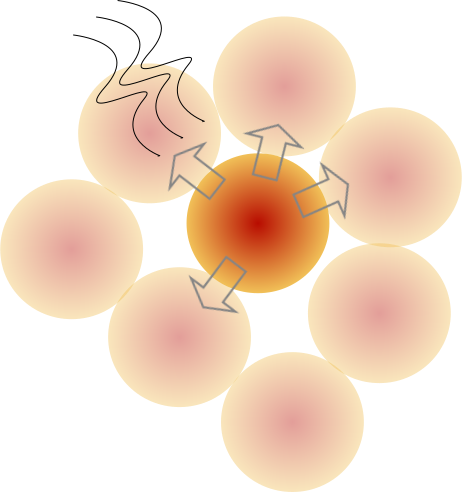
\includegraphics[width=0.75\textwidth]{chapters/figures/pebble-complete-heat-transfer}\label{fig:peb-comp-ht}
\end{figure}

Shown in Fig.~\ref{fig:peb-comp-ht} are all the modes of energy transfer on a pebble inside the fusion reactor. There is:

\begin{enumerate}
\item energy generated internal to the pebble caused by nuclear heating,
\item conduction internally of the solid material to the surface of the pebble, 
\item conduction between neighboring pebbles at their areas of contact, 
\item radiation between neighboring solids, and 
\item convective heat transfer with the interstitial helium gas (which includes energy carried far downstream or redeposited to neighboring pebbles).
\end{enumerate}









\subsection{Nuclear heating}

Nuclear deposition of energy is handled in a straightforward manner in the DEM computations with a simple source term on the energy balance equation. 












\subsection{Conduction through the solid}\label{sec:ht-pebble-conduction}

Before considering the heat equation in a sphere, it is instructive to first consider the simpler problem of a one-dimensional slab with volumetric heat generation, $q_g'''$ and convective cooling at the surfaces. The geometry is shown in Fig.~\ref{}.

Assuming we can find the Nusselt number for the convective cooling, we write the heat flux from the surface to the fluid as

\begin{equation}
	q_s'' = h(T_s - T_f)	
\end{equation}

where $T_f$ is the bulk fluid temperature and $T_s$ is the surface temperature. At steady-state the amount of heat moved across the fluid-surface interface must necessarily be equal to the total amount of heat generated into the slab. Therefore,

\begin{equation}
	q_w'' = q_g'''L = h(T_f-T_s)
\end{equation}

where $L$ is the half-width of the slab. For the sake of discussion, we re-write the above in terms of the temperature delta from surface to fluid in terms of nuclear heating,

\begin{equation}\label{eq:fluid-delta}
	T_f-T_s = \frac{q_g'''L}{h}
\end{equation}

Inside the slab, at steady-state the energy equation is simply a balance of heat conduction and nuclear generation. 

\begin{equation}\label{eq:nuclear-heating-slab-ode}
	0 = k\frac{\mathrm{d}^2T}{\mathrm{d}x^2} + q_g'''
\end{equation}

The boundary conditions are symmetry about the centerline and known surface temperature

\begin{align}
	q_{L=0} &= 0 \\
	T(L) &= T_s
\end{align}

The ODE of Eq.\ref{eq:nuclear-heating-slab-ode} is solved with simple separation and integration. When the boundary conditions are applied we have

\begin{equation}
	T(x) = \frac{q_g''' L^2}{2k}\left(1-\frac{x^2}{L^2}\right) + T_s
\end{equation}

We can find the temperature at the centerline of the slab, $x = 0$ as

\begin{equation}
	T_{cl} = \frac{q_g''' L^2}{2k} + T_s
\end{equation}

Or,

\begin{equation}\label{eq:centerline-delta}
	T_{cl} - T_s = \frac{q_g''' L^2}{2k}
\end{equation}

From Eqs.~\ref{eq:fluid-delta} and~\ref{eq:centerline-delta}, we see that the temperature differences between the surface and the fluid or the centerline and the surface are dictated by the heat generation rate relative to the speed at which that heat can be transported, via convection or conduction, respectively.

We will divide Eq.~\ref{eq:centerline-delta} by Eq.~\ref{eq:fluid-delta},

\begin{equation}\label{eq:biot-derivation}
	\frac{T_{cl} - T_s}{T_f-T_s} = \frac{1}{2}\frac{hL}{k}
\end{equation}

Careful observation of this equation can tell us much about the relative importance of the different modes of heat transfer to/from the surface. If the thermal transport away from the surface occurs at a much slower pace than thermal transport of energy through the solid to the surface, then the change in temperature across the solid $T_{cl}-T_{s}$ will be small compared to the change in temperature from the interface of solid to the bulkd fluid temperature, $T_{s}-T_f$. If the temperature across the solid is negligibly small in comparison to the surface-fluid difference, we are safe in the assumption that the solid is isothermal.

The group of terms on the right-hand-side of Eq.~\ref{eq:biot-derivation} is recognized as the Biot number,

\begin{equation}\label{eq:biot-number}
	\Bi=\frac{hL}{k}=\frac{R_{cond}}{R_{conv}}
\end{equation}

whose value is used to quantify the importance of internal conduction in the analysis of the solid interacting with convective heat transfer. If $\Bi<<1$, it is safely assumed that there is no temperature gradient in the solid material. A conclusion that will prove helpful in later analysis.

It is interesting to note that in this derivation of Biot number, we had considered nuclear heating as the source for temperature gradients across the pebble yet the rate of nuclear heating still does not appear in the Biot number. This implies that traditional assumptions of the validity of the lumped capacitance method hold even when dealing with a heat generation term in our energy balance.





\subsubsection{Large Biot number}

As we saw from the discussion of Eq.~\ref{eq:biot-number}, when the Biot number is small we can safely neglect temperature gradients through the solid we are analzying. However, when dealing with materials with low conductivity, i.e. larger $\Bi$, this assumption of negligible temperature gradient becomes decreasingly valid.  When dealing with spheres, there are slighty different accepted definitions of the Biot Number.  Some suggest that $\Bi=hd_p/6k$ is acceptable\cite{incropera:245}, where $d_p$ is the diameter of the particle.  However many use the more conservative definition of $\Bi=hd_p/2k$\cite{incropera:245,jeffreson409}.  For consistency and conservatism, we will proceed here with the latter definition.  

Considering now material and geometric properties relevant to our ceramic pebble beds, we will see that we may need to consider the effects of a larger $\Bi$ for our pebbles. The helium purge gas moving through the packed beds is not specifically intended to act as a heat transfer agent and moves along at a creeping flow rate. For a first approximation we will therefore assume as a lower limit the Nusselt number is $\Nu = 2$ (the value for a sphere in quiescent fluid). From the requirement that $\Bi \ll 1$, we have

\begin{equation}
	2 \frac{k_f}{k_s} \ll 1
\end{equation}

The conductivity of helium over the temperature range of 300 to 800 $^\circ$C is approximately 0.3 \si{W/m-K}. The solid conductivity of \lit and \lis are approximately 2 \si{W/m-K}. Because of the low conductivity of our solid, the Biot assumption is barely valid, $0.3 < 1$. 


































[Go back through Batchelor and O'Brien~\cite{Batchelor1977} paper]

\begin{equation}
	\frac{ k_s }{ k_f } \frac{a}{R^*} = \lambda
\end{equation}

Similar to the lumped capacitance assumptions, if $\lambda \gg 1$, the solid is approximately is isothermal. The second group on the left-hand side of this condition we remember from the assumptions of Hertz theory, where we require $\frac{a}{R^*} \ll 1^*$. Therefore to satisfy the condition of $\lambda \gg 1$, we require very large conductivity ratios of solid to fluid, $\frac{k_s}{k_f} \gg 1$. Alternatively this is satisfied by definition if the solids exist in vacuum.

Assuming that we satisfy the condition of isothermal solids, we address the conduction between solids in their small regions of contact.

[more details]










\subsection{Particle-particle conduction}

Handling the heat transfer between contacting particles has been investigated extensively by researchers in a number of fields\cite{Zhou2009,Zhang2011,Wu2011,Vargas2001,Li2000,Chaudhuri2006}. The amount of energy per time that can be transported per difference in temperature between pebble $i$ and $j$ as a conductance $h_{ij}$. Defined as

\begin{equation}\label{eq:pebble-conductance}
	\frac{h_{ij}}{k^*}= 2\left[\frac{3F_nR^*}{4E^*}\right]^{1/3}
\end{equation}

$k^*= 2k_ik_j/(k_i+k_j)$ is the effective solid conductivity of the two particles, and $F_n$ is the magnitude of the normal force between particles $i$ and $j$ as calculated by Eq.~\ref{eq:hertzForce}. Therefore, if we consider particles at temperatures $T_i$ and $T_j$ in contact, they will transfer heat at a rate of

\begin{equation}
	Q_{ij} = h_{ij}(T_i - T_j)
\end{equation} 











\subsection{Convection}











\subsection{Particle-particle radiation}
\section{Inter-particle heat conduction}\label{sec:ht-pebble-conduction}

Handling the heat transfer between contacting particles has been investigated extensively by researchers in a number of fields\cite{Zhou2009,Zhang2011,Wu2011,Vargas2001,Li2000,Chaudhuri2006}.

In the Hertz analysis we walked through in \S\ref{sec:hertz-contact}, we found the contact radius of two elastic spheres in Eq.~\ref{eq:hertz-radius} as a function of the contact pressure. We rewrite the radius in terms of the compression force acting on the bodies,

\begin{equation}
	a =  \left(\frac{3}{4}\frac{R^*}{E^*}\right)^{1/3}F^{1/3}	
\end{equation}

where $\frac{1}{E^*} = \frac{1-\nu_1^2}{E_1} + \frac{1-\nu_2^2}{E_2}$ and $\frac{1}{R^*} = \frac{1}{R_1} + \frac{1}{R_2}$ as before.

Batchelor and O'Brien\cite{Batchelor1977} made the brilliant observation that the temperature fields in the near-region of contacting spheres are analogous to the velocity potential of the potential flow of a fluid passing from from one reservoir to another through a circular hole in a planar wall. With the analogy, they could make use of the fluid flow solution to write the total flux across the circle of contact,

\begin{equation}\label{eq:pebble-conduction-heat-transfer}
	Q_{ij} = H_{ij}(T_i - T_j)
\end{equation}

with the heat conductance, 

\begin{equation}\label{eq:batchelor-pebble-conductance}
	H_{ij} = 2k_sa = 2k_s \left(\frac{3}{4}\frac{R^*}{E^*}\right)^{1/3}F^{1/3}
\end{equation}

governing the time rate of energy transferred per temperature difference between particles, $T_i$ and $T_j$, respectively. This approach, laid out by Batchelor and O'Brien, is valid when the thermal conductivity ratio of solid and fluid is well above unity and the contact area is small relative to the particle. The condition is expressed as,

\begin{equation}
	\frac{ k_s }{ k_f } \frac{a}{R^*} = \lambda \gg 1
\end{equation}

The model, being derived from Hertz theory, also carries with it many of the assumptions and limitations inherent with that theory. The assumptions are discussed in detail in \S\ref{sec:hertz-contact}.

Recently, Cheng, et al.\cite{Cheng19994199} proposed a slightly modified variant of the conductance given by Batchelor and O'Brien. In their model, they allow for contacting materials of different thermal conductivity. Therefore they have,

\begin{equation}
	H_{ij} = 2k^*a = 2k^* \left(\frac{3}{4}\frac{R^*}{E^*}\right)^{1/3}F^{1/3}
\end{equation}

where $\frac{1}{k^*} = \frac{1}{k_i} + \frac{1}{k_j}$. As well as being a more general, flexible formulation, the models analyzed by Cheng, et al.\cite{Cheng19994199} are in good agreement with experiments and will be used in this study.






\subsubsection{Large Biot number}
Considering now material and geometric properties relevant to our ceramic pebble beds, we will see that we may need to consider the effects of a larger $\Bi$ for our pebbles. The helium purge gas moving through the packed beds is not specifically intended to act as a heat transfer agent and moves along at a creeping flow rate. For a first approximation we will therefore assume as a lower limit the Nusselt number is $\Nu = 2$ (the value for a sphere in quiescent fluid). From the requirement that $\Bi \ll 1$, we have

\begin{equation}
	2 \frac{k_f}{k_s} \ll 1
\end{equation}

The conductivity of helium over the temperature range of 300 to 800 $^\circ$C is approximately 0.3 \si{W/m-K}. The solid conductivity of \lit and \lis are approximately 2 \si{W/m-K}. Because of the low conductivity of our solid, the Biot assumption is barely valid, $0.3 < 1$. 

\section{Nusselt number for spheres in packed beds}\label{sec:particle-convection}

%%%%%%%%%%%%%%%%%%%%%%%%%%%%%%%%%%%%%%%%%%










\subsection{Radiative transfer with neighboring particles}

The temperatures expected in the solid breeder are high enough that we can not a priori neglect radiation. The radiation exchange between contacting neighbors in a packed bed becomes extremely complex due to the local and semi-local nature of radiation. A standard approach to treat radiation exchange between surfaces is to consider the view factor between them. In a dense, randomly packed bed of spheres the computation of view factors between pebbles can be done via a method such as that proposed Feng and Han\cite{Feng2012}. Ideally, we could show this mode of heat transport is negligible compared to the others already discussed.

In ceramic breeder designs, the tritium breeding volume is rarely more than \si{2 cm} wide with pebbles that are, generally, \si{1 mm} in diameter. The maximum expected temperature in the breeding zone is about \si{1000 K}, roughly at the centerline of the \si{2 cm} width. The walls of the coolant must be held below the operable steel temperature of roughly \si{700 K}. This works out to a \si{300 K} differences spanning 10 pebble diameters. From this we can make a first-order approximation of \si{30 K} difference between neighboring pebbles. At the elevated temperatures, an estimate for the radiation exchange between two pebbles (allowing them to act as black bodies for this approximation) is

\begin{equation}
	\dot{Q}_\text{radiation} = \sigma A \left(T_\text{max}^4 - (T_\text{max}-30)^4\right) \approx 0.022\si{W}
\end{equation}
 
 which is the highest amount of radiation exchange we might expect between pebbles. 
